\documentclass[a4paper,twoside]{book}

\usepackage[utf8]{inputenc}
\usepackage[english,russian]{babel}
\usepackage{fontspec}
\setmainfont{Liberation Serif}
\setmonofont{Liberation Mono}

\usepackage{graphicx}
\renewcommand{\thefigure}{\thesection.\arabic{figure}}
\usepackage{hyperref}
\usepackage{multirow}
\usepackage[absolute,overlay,showboxes]{textpos}
\usepackage{etoolbox}
\usepackage{longtable}
\usepackage{tikz}
\usepackage{lilyglyphs}
\usepackage{tabularx}
\usepackage{pgfplots}
\usepackage{circuitikz}
\usepackage{minted}
\usepackage{glossaries}

\makeglossaries

\usepackage{svg}

\urlstyle{same}
\usepackage[printonlyused,withpage]{acronym}

\graphicspath{ {images/} {../images/} }

%% \documentclass[../main.tex]{subfiles}
%% \usepackage{svg}
%% \graphicspath{{\subfix{../images/}}}
%% \begin{document}

\newcounter{example-counter}
\setcounter{example-counter}{1}

%% This procedure adds the "Example" block to the text.
\newcommand{\example}[1]{
  \vspace{8pt}
  \begin{tabularx}{\textwidth}{m{1cm} m{9cm}}
    \includesvg[width=1.25cm]{the-noun-project/request-mirrored}
    & \textbf{Пример \arabic{example-counter}}: #1 \\
  \end{tabularx}
  \addtocounter{example-counter}{1}
}

\newcounter{experiment-counter}
\setcounter{experiment-counter}{1}

%% This procedure adds the "Experiment" block to the text.
\newcommand{\experiment}[2]{
  \vspace{8pt}
  \begin{tabularx}{\textwidth}{m{.15\textwidth}X m{.85\textwidth-4}X}
    \includesvg[width=1cm]{the-noun-project/flask}
    & \textbf{Эксперимент №\arabic{experiment-counter}:} #2 \\
  \end{tabularx}
  \addtocounter{experiment-counter}{1}
}

\newcommand{\note}[1]{
  \vspace{8pt}
  \begin{tabularx}{\textwidth}{m{1cm} m{9cm}}
    \includesvg[width=1cm]{the-noun-project/note}
    & \textbf{Примечание:} #1 \\
  \end{tabularx}
}

\newcommand{\hotkey}[1]{
  \texttt{#1}
}

%% This procedure allows to insert a music note.
%% Syntax:
%%   \musicnote{<octave>}{<note-name>}{<frequency>}
\newcommand{\musicnote}[3]{
  &
  \ifstrequal{#2}{C}{До   & C#1}{}
  \ifstrequal{#2}{D}{Ре   & D#1}{}
  \ifstrequal{#2}{E}{Ми   & E#1}{}
  \ifstrequal{#2}{F}{Фа   & F#1}{}
  \ifstrequal{#2}{G}{Соль & G#1}{}
  \ifstrequal{#2}{A}{Ля   & A#1}{}
  \ifstrequal{#2}{B}{Си   & B#1 (H#1)}{}
  & #3 \\
}

%% Taken from:
%%   <https://tex.stackexchange.com/questions/184923/how-to-include-a-second-file-only-if-environment-variable-is-set>
\newcommand{\newgetenv}[2][]{%
 \CatchFileEdef{\temp}{"|kpsewhich --var-value #2"}{\endlinechar=-1\relax}%
 \if\relax\detokenize{#1}\relax\temp\else\edef#1{\temp}\fi%
}%

\newcommand\esymbol[1]{%
  \begin{circuitikz}%
    \draw (0,0) to [#1] (1,0);%
  \end{circuitikz}%
}

\newcommand*{\soundWaveIcon}[0]{%
  \begin{tikzpicture}
    \draw[black, fill=black] (0, 0) circle (.25mm);
    \draw (.5mm, 0.7mm) arc (45:-45:1mm);
    \draw (1mm, 1mm) arc (45:-45:1.5mm);
    \draw (1.5mm, 1.3mm) arc (45:-45:2mm);
  \end{tikzpicture}%
}

%% \end{document}


\usepackage{subfiles}

%%%%%%%%%%%%%%%%%%%%%%%%%%%%%%%%%%%%%%%%%%%%%%%%%%%%%%%%%%%%%%%%%%%%%%%%%%%%%%%%
\title{Автомато-программато-компарадио-кружок}
\author{Артём ``avp'' Попцов\\\href{https://memory-heap.org}{memory-heap.org}}
\date{\today\\Версия 0.0.0}

\begin{document}

\maketitle

\tableofcontents

%%%%%%%%%%%%%%%%%%%%%%%%%%%%%%%%%%%%%%%%%%%%%%%%%%%%%%%%%%%%%%%%%%%%%%%%%%%%%%%%
\chapter*{Вступление}
\addcontentsline{toc}{chapter}{Вступление}

\subfile{sections/introduction.tex}

%%%%%%%%%%%%%%%%%%%%%%%%%%%%%%%%%%%%%%%%%%%%%%%%%%%%%%%%%%%%%%%%%%%%%%%%%%%%%%%%
\chapter{Основные принципы электротехники}

В первую очередь нам с вами надо рассмотреть базовые принципы того, как работает
электроника, чтобы впоследствии уметь собирать простые схемы.

Начнём с рассмотрения условий, которые необходимо выполнить, чтобы через
электрическую цепь шёл ток.

\subfile{sections/electronics-voltage}

\subfile{sections/electronics-circuits}

\subfile{sections/electronics-potential-difference}

\subfile{sections/electronics-resistance}

\subfile{sections/electronics-building-circuits}

%%%%%%%%%%%%%%%%%%%%%%%%%%%%%%%%%%%%%%%%%%%%%%%%%%%%%%%%%%%%%%%%%%%%%%%%%%%%%%%%
\chapter{Диалоги с компьютером}
\label{chapter:dialogues-with-computer}

\begin{figure}[ht]
  \centering
  \begin{tikzpicture}
    %% Display.
    \node[rectangle,
      rounded corners = 0.2,
      draw = black,
      minimum width = 3cm,
      minimum height = 2cm] (r) at (1, 2) {Hello, World!};

    \node[rectangle,
      thick,
      rounded corners = 0.25cm,
      draw = black,
      minimum width = 4cm,
      minimum height = 3cm] (r) at (1.25, 2) {};

    %% Display Knobs.
    \node[circle, draw, radius = 0.1cm] (c) at (2.85, 2.0) {};
    \node[circle, draw, radius = 0.1cm] (c) at (2.85, 1.6) {};
    \node[circle, draw, radius = 0.1cm] (c) at (2.85, 1.2) {};

    %% Display Legs.
    \node[rectangle,
      thick,
      draw = black,
      minimum width = 0.2cm,
      minimum height = 0.19cm] (r) at (0, 0.38) {};

    \node[rectangle,
      thick,
      draw = black,
      minimum width = 0.2cm,
      minimum height = 0.19cm] (r) at (2.25, 0.38) {};

    %% System Case.
    \node[rectangle,
      thick,
      rounded corners = 0.25cm,
      draw = black,
      minimum width = 5.5cm,
      minimum height = 1.5cm] (r) at (0.75, -0.48) {};

    %% Floppy Drives.
    \node[rectangle,
      draw = black,
      minimum width = 2cm,
      minimum height = 1.25cm] (r) at (2.25, -0.36) {};

    \node[rectangle,
      draw = black,
      minimum width = 1.75cm,
      minimum height = 0.5cm] (r) at (2.25, -0.1) {};

    \node[rectangle,
      draw = black,
      minimum width = 1.75cm,
      minimum height = 0.5cm] (r) at (2.25, -0.6) {};

    \draw[very thick] (1.5, -0.15) -- (3, -0.15);

    \draw[very thick] (1.8, -0.6) -- (2.7, -0.6);

    %% Control buttons.
    \node[rectangle,
      draw = black,
      minimum width = 1cm,
      minimum height = 0.25cm] (r) at (-0.4, -0.25) {};

    %% Ventilation holes in the case.
    \foreach \offset in {0.1, 0.2, ..., 2.6} {
      \draw[thick] (-1.8 + \offset, -1) -- (-1.8 + \offset, -0.5);
    };

  \end{tikzpicture}
\end{figure}

\subfile{sections/dialogues-with-computer-introduction}

\subfile{sections/dialogues-with-computer-algorithms}

\subfile{sections/dialogues-with-computer-arduino}

%%%%%%%%%%%%%%%%%%%%%%%%%%%%%%%%%%%%%%%%%%%%%%%%%%%%%%%%%%%%%%%%%%%%%%%%%%%%%%%%
\section{Работа с макетной платой}

Макетная плата позволяет собирать схемы (подключать электронику) без применения
пайки --- это упрощает прототипирование и ускоряет процесс разработки проектов.
Компоненты просто вставляются в слоты на макетной плате для соединения
(см. рис. \ref{fig:breadboard-led}.)

\begin{figure}[ht]
  \centering
  \caption{Пример подключения светодиода к Arduino Mega 2560 через макетную
    плату.}
  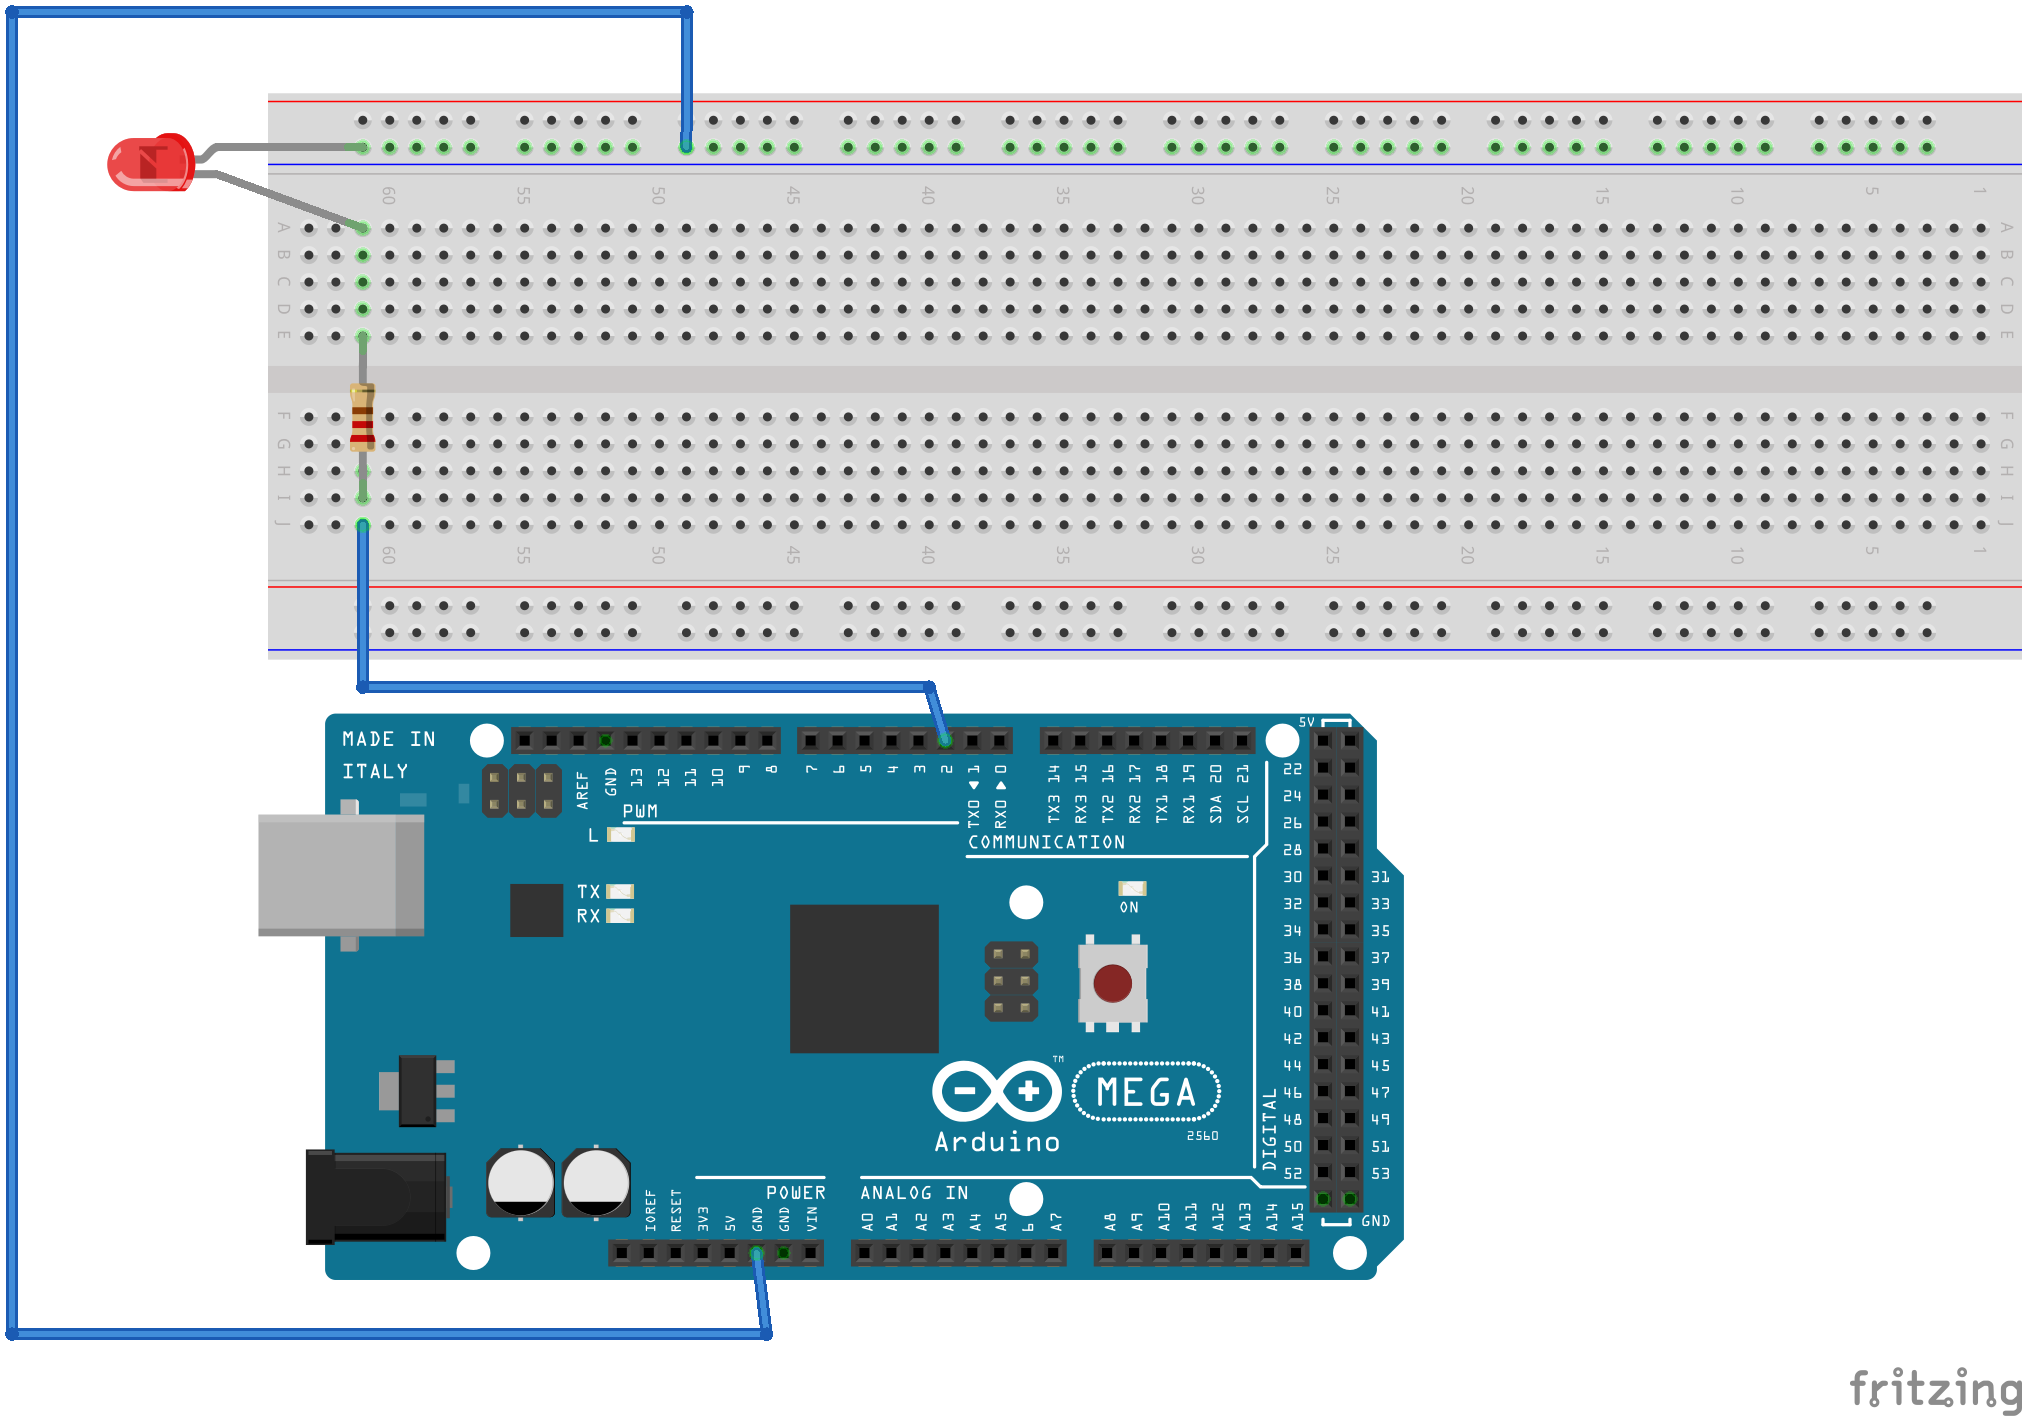
\includegraphics[width=12cm]{schematics/001-led}
  \label{fig:breadboard-led}
\end{figure}

\begin{itemize}
\item Черный провод подключен к arduino и идёт на вывод GND (минус)
\item Синий провод подключен к arduino и идёт на вывод 5V (плюс)
\end{itemize}

\note{ Обратите внимание, что светодиоды (и некоторые другие элементы)
  подключаются к платформе Arduino через резистор -- это необходимо для
  обеспечения бесперебойной работы схемы и предупреждения всяческих поломок и
  ухудшения работы как отдельных деталей, так и схемы в целом.  }

\section{Подключение Arduino к компьютеру}
Чтобы подключить ардуино к компьютеру вам потребуется сама платформа Arduino (в
нашем случае мы используем Arduino Mega 2560) и кабель стандарта USB-В.

Соедините Arduino с компьютером через USB-кабель. Вы увидите, как на плате
загорится светодиод ``ON''.

Теперь необходимо настроить Arduino IDE для работы с подключенной Arduino, для
этого нужно войти в панель ``Инструменты'' затем ``Плата'' -- в этом меню
выберите 6Arduino с которой вы сейчас работаете, затем в подменю ``Порт''
выберите порт, к которому подключена Arduino.

\newpage
\subfile{sections/dialogues-with-computer-arduino-ide}

\subfile{sections/dialogues-with-computer-program-structure}

\subfile{sections/dialogues-with-computer-memory}

\subfile{sections/dialogues-with-computer-control-flow}

%%%%%%%%%%%%%%%%%%%%%%%%%%%%%%%%%%%%%%%%%%%%%%%%%%%%%%%%%%%%%%%%%%%%%%%%%%%%%%%%
\chapter{Белый шум}

\subfile{sections/white-noise-introduction}
\subfile{sections/white-noise-signal-types}
\subfile{sections/white-noise-serial-port}
\subfile{sections/white-noise-analog-ports}
\subfile{sections/white-noise-adc}

%%%%%%%%%%%%%%%%%%%%%%%%%%%%%%%%%%%%%%%%%%%%%%%%%%%%%%%%%%%%%%%%%%%%%%%%%%%%%%%%
\chapter{Широтно-импульсная модуляция}

\subfile{sections/pwm-intro}
\subfile{sections/pwm-wavelength}
\subfile{sections/pwm-duty-cycle}


%%%%%%%%%%%%%%%%%%%%%%%%%%%%%%%%%%%%%%%%%%%%%%%%%%%%%%%%%%%%%%%%%%%%%%%%%%%%%%%%
\subsection{Задачи}

\begin{enumerate}
\item Написать программу, плавно включающую и выключающую светодиод. Собрать и
  протестировать схему. 
\item Написать программу, реализующую ``бегущий огонь'' с использованием ШИМ.
  Собрать и протестировать схему.
\item Используя потенциометр, модифицировать систему из задания №2 таким
  образом, чтобы можно было регулировать яркость ``бегущего огня''.
\item Разработать ``бегущий огонь'', где следующий светодиод начинает плавно
  разгораться одновременно с затуханием предыдущего светодиода.
\end{enumerate}

%% \section{Последовательный порт}

%% \subsection{Сбор и обработка данных на стороне компьютера}

%% Другой задачей, решаемой с помощью функций записи данных в последовательный
%% порт, является сбор данных на стороне компьютера. Arduino IDE позволяет нам
%% визуализировать данные через специальный плоттер (доступ к которому можно
%% получить, выбрав в меню ``Инструменты'' пункт ``Плоттер по последовательному
%% соединению'', либо нажав комбинацию клавиш \hotkey{Ctrl + Shift + L}.)

%% \subsection{Передача данных с компьютера на Arduino}

%% Передавать данные с Arduino на компьютер мы уже научились. Теперь посмотрим на
%% передачу данных в обратном направлении. Для того чтобы передать данные с
%% компьютера на Arduino также необходимо выполнить настройку последовательного
%% порта; кроме этого, нам потребуется задействовать несколько новых функций.

%% \subsubsection{Чтение отдельных байт}

%% Функция \texttt{Serial.read} читает байт данных из поступивших на Arduino. То
%% есть возвращает вам некое целое число, с которым вы вольны делать что вашей душе
%% угодно. Каждый вызов этого метода будет возвращать вам следующий байт данных из
%% тех что поступили на Arduino. Если возвращать нечего, то есть вы считали все что
%% было, данная функция вернет -1.

%% \note{ Если передаются именно байты, возникает проблема: -1 это 0xFF в
%%   шестнадцатиричной системе, или 255 в десятичной. Такой же байт, как и все
%%   остальные, из-за чего невозможно. поэтому нужно сперва вызывать функцию available . }

%% Допустим мы отправили 1 байт данных на Arduino и использовали нижеприведенный
%% участок кода:

%% \begin{verbatim}
%% int incoming_byte;
%% void loop() {
%%   if (Serial.available() > 0) {
%%       incoming_byte = Serial.read();
%%   }
%% }
%% \end{verbatim}

%% После того, как вы считаете байт данных, он будет перемещен в вашу переменную
%% \texttt{incoming\_byte} а функция \texttt{Serial.available} снова будет
%% возвращать 0, пока не поступят новые данные.

%% То есть, когда вы считываете байт, показания счетчика принятых байт уменьшается
%% и \texttt{Serial.available} будет показывать на 1 байт меньше.

%% Помните, что функция \texttt{Serial.read} возвращает только 1 байт данных, если
%% например вы передали 4 символа каждый по 1 байту, вам потребуется 4 раза вызвать
%% данную функцию чтобы прочитать эти символы и самостоятельно позаботится о том
%% чтобы разместить их в массив символов либо воспользоваться функцией
%% \texttt{Serial.readBytes}.

%% \subsubsection{Чтение чисел}

%% Функция \texttt{Serial.parseInt} просматривает данные, поступившие на Arduino, и
%% ищет среди них набор кодов (чисел) от 48 до 57, которые соответствуют символам
%% чисел от 0 до 9 и преобразует все это в правильное целочисленное значение. Таким
%% образом если вы с монитора порта передадите "число" (на самом деле, строку)
%% ``72'', данный метод увидит 2 последовательных байта 55 и 51, корректно
%% преобразует его в число 72 и вернет его как правильное целочисленное значение.
%% Давайте напишем маленькую эхо-программу, которая покажет принцип работы данной
%% функции и позволит вам узнать какому символу соответствует то или иное число.

%% \begin{verbatim}
%% int incoming_int = 0;

%% void setup()
%% {
%%   Serial.begin(9600);
%%   Serial.setTimeout(2000);
%% }
%% void loop()
%% {
%%   if (Serial.available() > 0)
%%   {
%%     incoming_int = Serial.parseInt();
%%     Serial.write(incoming_int);
%%   }
%% }
%% \end{verbatim}

%% Данная программа будет работать так. Если в мониторе порта вы введете строку
%% ``72'' то монитор порта отправит его на Arduino как два байта данных в виде
%% чисел 55 и 51, функция \texttt{Serial.parseInt} подождет 2000 миллисекунд (как
%% видите я поменял время ожидание с 1 секунды на 2 секунды, чтобы нагляднее
%% показать кое какие аспекты) увидит эти два значения и преобразует их в одно
%% целочисленное 72 и присвоит его переменной \texttt{incoming\_int}, мы с помощью
%% метода \texttt{Serial.write} передадим число 72 как есть обратно в монитор порта
%% (почему именно этот метод нужен читайте далее) где монитор порта корректно
%% преобразует число 72 в соответствующий символ и покажет нам символ ``H'' который
%% соответствует коду 72. Таким образом мы можем передавать числовые значения с
%% компьютера на платформу Arduino и дальше использовать эти значения.

\chapter{Синтез музыки и технологии}

\subfile{sections/music-and-technology-synthesis-sound}
\subfile{sections/music-and-technology-synthesis-speaker}
\subfile{sections/music-and-technology-synthesis-rhythm}
\subfile{sections/music-and-technology-synthesis-harmony}
\subfile{sections/music-and-technology-synthesis-octave-system}
\subfile{sections/music-and-technology-synthesis-simple-melodies}
\subfile{sections/music-and-technology-synthesis-arrays}
\subfile{sections/music-and-technology-synthesis-two-dimensional-arrays}

%%%%%%%%%%%%%%%%%%%%%%%%%%%%%%%%%%%%%%%%%%%%%%%%%%%%%%%%%%%%%%%%%%%%%%%%%%%%%%%%
\section{Паузы в музыке}

Есть ещё один момент, на котором мы до текущего момента не заостряли внимание ---
паузы в произведении. Правильные паузы также важны, как и сами ноты.

В нотной записи паузы отмечаются специальными значками (см. рисунок
\ref{fig:lilypond-rest-example-1}.) \footnote{В музыке существуют паузы,
занммающие несколько тактов, либо очень короткие паузы -- тридцать вторые,
шестьдесят четвёртые и т.п. Используются они редко, поэтому мы их не будем
разбирать здесь.}

\begin{figure}[ht]
  \caption{Паузы в музыке.}
  \centering
  \begin{lilypond}
    \relative c' {
      \numericTimeSignature
      \time 4/4
      r1-"Целая."
    }
  \end{lilypond}
  \begin{lilypond}
    \relative c' {
      \numericTimeSignature
      \time 4/4
      r2-"Половинная." r2
    }
  \end{lilypond}
  \begin{lilypond}
    \relative c' {
      \numericTimeSignature
      \time 4/4
      r4-"Четвертная." r4 r4 r4
    }
  \end{lilypond}
  \begin{lilypond}
    \relative c' {
      \numericTimeSignature
      \time 4/4
      r8-"Восьмая." r8 r8 r8 r8 r8 r8 r8
    }
  \end{lilypond}
  \begin{lilypond}
    \relative c' {
      \numericTimeSignature
      \time 4/4
      r16-"Шестнадцатая." r16 r16 r16
      r16 r16 r16 r16
      r16 r16 r16 r16
      r16 r16 r16 r16
    }
  \end{lilypond}
  \label{fig:lilypond-rest-example-1}
\end{figure}

Целая пауза равна по длине целой ноте, половинная --- половине целой ноты и т.д.
Иными словами, мы можем использовать подход, примененный нами для высчитывания
длительности нот, для расчета длительности пауз в произведении.

Обозначения пауз с их длительностями предтсавлены в таблице
\ref{table:music-rest-legths}.

\begin{table}[ht]
  \caption{Некоторые возможные длительности пауз.}
  \begin{tabular}{p{3cm}|p{4cm}|p{3.5cm}}
    Начертание & Длительность & Название \\
    \hline \hline
    \wholeNoteRest     & $\frac{1}{1}$ & ``Целая'' \\
    \hline
    \halfNoteRest      & $\frac{1}{2}$ & ``Половина'' \\
    \hline
    \crotchetRest        & $\frac{1}{4}$ & ``Четверть'' \\
    \hline
    \quaverRest    & $\frac{1}{8}$ & ``Восьмая'' \\
    \hline
    \semiquaverRest & $\frac{1}{16}$ & ``Шестнадцатая'' \\
    \hline
  \end{tabular}
  \label{table:music-rest-legths}
\end{table}

Для реализации паузы в программе необходимо во-первых создать специальную ноту с
нулевой частотой. Пауза в музыке называется ``Покой'' (или ``Rest''
по-английски), поэтому для обозначения паузы в программе мы будем использовать
заглавную букву ``R''.

\begin{verbatim}
const float R = 0; // Пауза ("Rest")
\end{verbatim}

Далее нам необходимо изменить функцию \texttt{play\_tone} таким образом, чтобы
она могла корректно ``воспроизводить'' паузы. Для этого нам необходимо добавить
такое условие, чтобы, если частота ноты больше нуля, то функция выполняла тот
код, который мы использовали раньше; иначе -- чтобы выполнялась просто задержка.

\begin{minted}{cpp}
// Функция воспроизведения звука указанной частоты.
void play_tone(int port, float f, long t) {
  if (f > 0) {
    const int T = 1000000 / f;
    int d = T / 2;
    int count = t / T;
    for (int i = 0; i < count; i++) {
      digitalWrite(port, HIGH);
      delayMicroseconds(d);
      digitalWrite(port, LOW);
      delayMicroseconds(d);
    }
  } else {
    delay(t / 1000); // Пауза
  }
}
\end{minted}

Обратите внимание, что для создания задержки мы используем код \texttt{delay(t /
  1000)} -- делить \texttt{t} на 1000 необходимо по той причине, что время
проигрывания ноты (\texttt{t}) задаётся в микросекундах, а функция
\texttt{delay} принимает время ожидания в миллисекундах. Чтобы преобразовать
микросекунды в миллисекунды, достаточно поделить количество микросекунд на 1000
(так как в каждой микросекунде содержится 1000 миллисекунд.) Почему же мы не
могли использовать функцию \texttt{delayMicroseconds} для организации задержек
(пауз) прямо в микросекундах, без преобразования? Ответ прост --
\texttt{delayMicroseconds} не умеет долго ждать, и значения \texttt{t} для неё
будут слишком большими; если мы попытаемся использовать
\texttt{delayMicroseconds} с большими отрезками времени, то она не будет
корректно их обрабатывать, и задержка получится неправильной.

Для наглядной демонстрации использования пауз возьмём другое музыкальное
произведение -- ``Кабы небыло зимы'' из мультфильма ``Простоквашино''.

\begin{figure}[ht]
  \caption{Часть мелодии ``Кабы небыло зимы'' из мультфильма ``Простоквашино''.}
  \begin{lilypond}
    \relative c' {
      \key g \major
      \numericTimeSignature
      \time 4/4
      b8 b b'8. fis16 a8 g e4 |
      d8 d << b'8. d8. >> << c16 a >> << c8 a >> << b8 g8 >> r4
      d'8 c a fis << a c >> << g b >> << g4 b >>
      b,8 b << g'8. b8. >> << fis16 a >> << fis8 a >> << e8 g8 >> r4
    }
    \layout {
      indent = 0\mm
      line-width = 120\mm
      ragged-last = ##t
    }
  \end{lilypond}
  \label{fig:lilypond-melody-prostokvashino}
\end{figure}

В нотной записи на рисунке \ref{fig:lilypond-melody-prostokvashino} представлена
часть мелодии, которую мы попытаемся переложить на программный код. Полную
версию мелодии можно увидеть на рисунке
\ref{fig:lilypond-melody-prostokvashino-full}.

Можно заметить две четвертные паузы (\crotchetRest), которые необходимо добавить
в массив нот, чтобы произведение звучало, как в оригинале.

Можно также заметить двойные ноты, записанные одна над другой -- это значит, что
данные ноты должны играться одновременно. Для упрощения нашей задачи мы пока
будем брать самую верхнюю ноту из группы.

Попробуем вписать ноты в массив и послушать, как они будут звучать. Чтобы не
запутаться, разобъём ноты по группам, согласно тактам (по одной группе на
строке) -- а рядом с каждой группой в виде комментария напишем номер этого такта
(например, такт номер ноль мы пометили \texttt{/* 0 */}.)

\begin{minted}{cpp}
float prostokvashino[28][2] = {
  /* 0 */ {b3, 8}, {b3, 8}, {b4, 8}, {f4, 16}, {a4, 8}, {g4, 8}, {e4, 4},
  /* 1 */ {d4, 8}, {d4, 8}, {d5, 8}, {c5, 16}, {c5, 8}, {b4, 8}, {R,  4},
  /* 2 */ {d5, 8}, {c5, 8}, {a4, 8}, {f4, 8},  {c5, 8}, {b4, 8}, {b4, 4},
  /* 3 */ {b3, 8}, {b3, 8}, {b4, 8}, {a4, 16}, {a4, 8}, {g4, 8}, {R,  4},
};
\end{minted}

При воспроизведении мелодия будет похожей на оригинал, однако вы можете заметить
некоторые ``несоответствия''. Источников данных несоответствий несколько. Первый
источник проблем в том, мы не учитываем, что длительность некоторых нот, которые
помечены точкой справа (вот так: ``\eighthNoteDotted'') больше стандартной.

%%%%%%%%%%%%%%%%%%%%%%%%%%%%%%%%%%%%%%%%%%%%%%%%%%%%%%%%%%%%%%%%%%%%%%%%%%%%%%%%
\section{Ноты с точками}

В музыкальной нотации точка, которая ставится справа от ноты, увеличивает её
длительность на половину от базовой.

Например, если у нас точка идёт после восьмушки (``\eighthNoteDotted''), то
следовательно к её длительности будет прибавляться половина от её длительности.
Половинка от восьмушки -- это шестнадцатая. Чтобы сложить простые дроби, которые
у нас получились, необходимо привести их к общему знаменателю. И формула
вычисления длительности будет следующая:

\begin{equation}
  \mbox{\eighthNoteDotted} = \mbox{\eighthNote} + \mbox{\sixteenthNote}
  = \frac{1}{8} + \frac{1}{16} = \frac{2}{16} + \frac{1}{16} = \frac{3}{16}
\end{equation}

Получившееся число $\frac{3}{16}$ для нас неудобно, так как мы в программе
подставляем в числитель дроби длительность одного такта, а тут у нас получается,
что необходимо поставить длину трёх тактов. Чтобы избавиться от этой неудобной
тройки в числителе, мы можем разделить числитель и знаменатель на 3.

\begin{equation}
  \frac{3 / 3}{16 / 3} = \frac{1}{16 / 3}
\end{equation}

Получившееся число $16 / 3$ необходимо подставить в массив с нашими нотами.
Например, третья нота нулевого такта -- ``B4'' -- как раз восьмая с точкой. В
массиве её длительность надо исправить -- вместо \texttt{\{b4, 8\}} написать
\texttt{\{b4, 16.0 / 3.0\}}. Тоже самое необходимо сделать с другими нотами,
возле которых стоит точка.

Для того, чтобы даннй код уместился в книгу, нам пришлось разбить каждый такт на
две строки, но по комментариям и отступам должно быть понятно, что происходит в
коде.

\begin{minted}{cpp}
float prostokvashino[28][2] = {
  /* 0 */ {b3, 8},  {b3, 8}, {b4, 16.0 / 3.0},
  /*   */ {f4, 16}, {a4, 8}, {g4,          8}, {e4, 4},
  /* 1 */ {d4, 8},  {d4, 8}, {d5, 16.0 / 3.0},
  /*   */ {c5, 16}, {c5, 8}, {b4,          8}, {R,  4},
  /* 2 */ {d5, 8},  {c5, 8}, {a4,          8},
  /*   */ {f4, 8},  {c5, 8}, {b4,          8}, {b4, 4},
  /* 3 */ {b3, 8},  {b3, 8}, {b4, 16.0 / 3.0},
  /*   */ {a4, 16}, {a4, 8}, {g4,          8}, {R,  4},
};
\end{minted}

Теперь наша мелодия звучит ещё более похоже на оригинал.

Здесь стоит упомянуть, что в музыке встречаются ноты двумя точками справа, что
даёт удлинение ноты на половину её длительности и на половину от половины -- но
подобные ситуации редки из-за неудобства рассчёта необходимой длительности при
чтении музыкантом нот с листа. То ли дело нам, программистам -- прочитали
неспеша, запрограммировали, а там пусть компьютер сам пыжится над нашим
творением!

%%%%%%%%%%%%%%%%%%%%%%%%%%%%%%%%%%%%%%%%%%%%%%%%%%%%%%%%%%%%%%%%%%%%%%%%%%%%%%%%
\section{Полутона, диезы и бемоли}

Мы с вами всю эту главу говорим, что нот в октаве семь, и суммарно звуков 63
штуки, если считать по всем октавам. Но это не совсем точно -- на самом деле
звуков в октаве не семь, а двенадцать!

Вот так сюрприз. Откуда берутся дополнительные пять звуков? Оказывается, что в
музыке есть так называемые \emph{полутона}, которые позволяют разнообразить
музыку новыми звуками.

Нагляднее всего эти скрытные звуки легче всего увидеть на клавиатуре пианино.

\begin{figure}[ht]
  \caption{Одна октава на клавиатуре пианино.}
  \centering
  \begin{tikzpicture}
    \draw (0, 0) -- (7, 0);
    \foreach \x/\note in {0/C, 1/D, 2/E, 3/F, 4/G, 5/A, 6/B, 7/} {
      \draw (\x, 0) -- (\x, 2) -- (\x, 0) node[anchor=south west] {\note};
    };
    \foreach \x in {1, 2, 4, 5, 6} {
      \node[
        rectangle,
        draw,
        fill=black,
        minimum width=0.5cm,
        minimum height=1.35cm
      ] (r) at (\x, 1.30) {};
    };
  \end{tikzpicture}
  \label{fig:lilypond-music-graph-1}
\end{figure}

Видно, что между парами нот ``C''--``D'', ``D''--``E'', ``F''--``G'',
``G''--``A'', ``A''--``B'' находятся чёрные клавиши. Если мы посчитаем, сколько
всего клавиш в одной октаве, то получим двенадцать штук -- двенадцать звуков.

Объясняется это тем, что между двумя соседними клавишами \emph{расстояние в один
полутон}, если представить частотный диапазон октавы как некий отрезок.
Большинство пар нот имеют друг от друга достаточное расстояние, чтобы туда,
ровно посерёдке, добавить ещё одну клавишу (исключение составляют пары
``B''--``C'', ``E''--``F''.)

Каких-то особых закорючек для этих дополнительных звуков в музыке не
применяется, однако есть ``модификаторы'' для основных семи нот, поднимающих или
понижающих их частоту на полутон.

Для того, чтобы например получить частоту клавиши между парой ``C''--``D'',
можно поднять частоту ``C'' на пол-тона, либо понизить частоту ``D'' на те же
пол-тона.

Модификатор, повышающий частоту ноты на пол-тона называется \emph{диезом}, тогда
как аналогичный модификатор, понижающий частоту на пол-тона, называется
\emph{бемолем}.

Ноты с модификатором ``Диез'' помечаются решёткой (``\#''), стоящей перед нотой
-- например, на рис. \ref{fig:lilypond-f4-sharp} изображена ``Фа Диез''
четвёртой октавы.

\begin{figure}[ht]
  \caption{``Фа Диез'' четвёртой октавы.}
  \centering
  \begin{lilypond}
    \relative c' {
      \numericTimeSignature
      \time 4/4
      fis4
    }
  \end{lilypond}
  \label{fig:lilypond-f4-sharp}
\end{figure}

Чтобы высчитать частоту ``F4\#'', надо найти среднее арифметическое для частот
ноты ``F4'' и следующей перед ней ноты ``G4'' (см. формулу
\ref{quation:f-sharp-calculation}.)

\begin{equation}
  \frac{\mbox{F4} + \mbox{G4}}{2} = \mbox{F4\#}
  \label{quation:f-sharp-calculation}
\end{equation}

Программно вычислить ``F4\#'' не составляет труда, как показано в коде ниже.
Заметьте, что мы обозначили получившуюся частоту, как \texttt{f4s}, так как ``Фа
Диез'' по-английски пишется, как ``Fa Sharp'', и мы используем букву ``s'' из
слова ``sharp'' после ноты для краткости.

\begin{minted}{cpp}
const float f4  = 349.230;
const float g4  = 392.000;
const float f4s = (f4 + g4) / 2; // F4 Диез
\end{minted}

Подобный подход работает и с другими нотами.

Кстати, для тех нот, после которых нет чёрной клавиши (``B'', ``E''), диезом
является просто следующая нота -- например, ``E4\#'' -- это ``F4'', а ``B4\#'' не
что иное, как ``C5''.

Таким образом:

\begin{minted}{cpp}
const float e4  = 329.630;
const float f4  = 349.230;
const float e4s = f4; // E4 Диез
\end{minted}

Бемоли по логике работают схоже с диезами, с одним отличием -- они
\textbf{понижают} частоту ноты на половину тона. Обозначаются бемоли специальным
символом ``\flat'', который ставится перед нотой, на которую ``накладывается''
модификатор ``бемоль''.

Для примера возьмём ``E4\flat'' (см. рисунок \ref{fig:lilypond-e4-flat}.)

\begin{figure}[ht]
  \caption{``Фа Диез'' четвёртой октавы.}
  \centering
  \begin{lilypond}
    \relative c' {
      \numericTimeSignature
      \time 4/4
      ees4
    }
  \end{lilypond}
  \label{fig:lilypond-e4-flat}
\end{figure}

Бемоль для неё -- это частота ровно посерёдке между ``E4'' и предыдущей нотой от
неё (``D4''), как показано на формуле \ref{equation:e-flat-calculation}.

\begin{equation}
  \frac{\mbox{E4} + \mbox{D4}}{2} = \mbox{E4\flat}
  \label{equation:e-flat-calculation}
\end{equation}

Для обозначения бемолей в программном коде мы будем добавлять букву ``f'' к
имени ноты, после её номера октавы, так как в английском ноты с бемолями
называются ``приплюcнутыми'' (``flat'') -- например, ``E4 Бемоль'' будет
называться ``E4 Flat''.\footnote{В музыке иногда встречатеся двойные диезы и
двойные бемоли, что означает необходимость брать ноту на два полутона выше или
ниже -- по сути, брать следующую или предыдующую ноту.}

\begin{minted}{cpp}
const float d4  = 293.660;
const float e4  = 329.630;
const float e4f = (e4 + d4) / 2; // E4 Бемоль
\end{minted}

Все эти диезы и бемоли мы пока с вами рассматривали в вариантах, когда
знак-модификатор пишется разу перед нотой, на которую ``накладывается
заклинание'' -- они называются знаками ``по-месту'', или ``случайными'' (англ.
\emph{accidentals}.) Но музыкантам неудобно писать подобные модификаторы перед
каждой нотой, если подобных случаев в композиции много. Чтобы решить эту
проблему, в музыке используются знаки диезов и бемолей, которые ставятся в
начале нотного стана -- в начале линий нотоносца. Влияние таких значков
распространяется на все ноты подобные той, на которую наложено ``заклинание''.

Вернёмся к мелодии ``Кабы небыло зимы''.  Если посмотреть на начало каждой
строки, то можно увидеть решёнку на ``F5'' -- это означает, что все ноты ``F''
будут диезами.

\begin{tikzpicture}
  \node (image) at (4, 0) {
    \begin{lilypond}
      \relative c' {
        \key g \major
        \numericTimeSignature
        \time 4/4
        b8 b b'8. fis16 a8 g e4 |
        d8 d << b'8. d8. >> << c16 a >> << c8 a >> << b8 g8 >> r4
      }
      \layout {
        indent = 0\mm
        line-width = 120\mm
        ragged-last = ##t
      }
    \end{lilypond}
  };
  \draw[red, thick, ->] (0.0, 1.0) node[anchor=south west] {F5 Диез} -- (-0.5, 0.5);
  \label{fig:lilypond-melody-prostokvashino-2}
\end{tikzpicture}

Зная это, мы можем соответствующим образом модифицировать код нашей мелодии.

\begin{minted}{cpp}
const float f4s = (f4 + g4) / 2;

// ...

float prostokvashino[28][2] = {
  /* 0 */ {b3,  8},  {b3, 8}, {b4, 16.0 / 3.0},
  /*   */ {f4s, 16}, {a4, 8}, {g4,          8}, {e4, 4},
  /* 1 */ {d4,  8},  {d4, 8}, {d5, 16.0 / 3.0},
  /*   */ {c5,  16}, {c5, 8}, {b4,          8}, {R,  4},
  /* 2 */ {d5,  8},  {c5, 8}, {a4,          8},
  /*   */ {f4s, 8},  {c5, 8}, {b4,          8}, {b4, 4},
  /* 3 */ {b3,  8},  {b3, 8}, {b4, 16.0 / 3.0},
  /*   */ {a4,  16}, {a4, 8}, {g4,          8}, {R,  4},
};

// ...
\end{minted}

%%%%%%%%%%%%%%%%%%%%%%%%%%%%%%%%%%%%%%%%%%%%%%%%%%%%%%%%%%%%%%%%%%%%%%%%%%%%%%%%
\section{Музыкальный размер}

Вы могли видеть, что на нотном стане в самом начале, возле скрипичного (или
басового) ключа часто написано $\frac{4}{4}$ -- что же это означает?

Пометка $\frac{4}{4}$ (читается как ``четыре четверти'') обозначает
\emph{музыкальный размер} произведения.  С точки зрения кодирования мелодии в
программе это не влияет ни на частоту нот, ни на их длительность.  При этом,
однако, данная пометка напрямую влияет на звучание произведения, и без её учёта
все произведения будут звучать ``плоско'' и менее интересно.

Удивительный эффект музыкальный размер даёт благодаря \emph{акцентированию}
определённых нот.

Например, посмотрим ещё раз на ``Twinkle, Twinkle, Little Star''
(\ref{fig:lilypond-musical-scale-example-1}.)

\begin{figure}[ht]
  \caption{``Twinkle, Twinkle, Little Star'' в размере четыре четверти.}
  \centering
  \begin{lilypond}
    \relative c' {
      \numericTimeSignature
      \time 4/4
      c4 c g' g
      a a g2
      f4 f e e
      d d c2
      g'4 g f f
      e e d2
      g4 g f f
      e e d2
      c4 c g' g
      a a g2
      f4 f e e
      d d c2
    }
    \layout {
      indent = 0\mm
      line-width = 100\mm
      ragged-last = ##t
    }
  \end{lilypond}
  \label{fig:lilypond-musical-scale-example-1}
\end{figure}

Поскольку композиция записана в музыкальном размере ``четыре четверти'', то в
один такт убирается ровно четыре четвёртных ноты, или суммарно единица (или одна
целая нота.)  Числитель данной дроби указывает, сколько частей -- или, по-другому
называемые \emph{долей} -- убирается в такт.  Знаменатель дроби указывает, на
какие именно доли делится такт.  В размере ``четыре четверти'' такт делится на
четыре части по одной четвертной ноте.

При игре музыкального произведения на каком-либо инструменте акцент идёт обычно
на первую ноту из такта -- на её \emph{сильную долю}.  Доли, которые не
акцентированы, называются \emph{слабыми долями}.

С точки зрения исполнения акцентированные ноты должны звучать громче, или
каким-либо другим способом выделяться в общем звучании.

Акцент нот обозначается значком ``>'' над (или под) нотой.  Если мы расставим
значки, обозначающие акцент, то получим следующую запись
(см. рис. \ref{fig:lilypond-musical-scale-example-2}.)

\begin{figure}[ht]
  \caption{``Twinkle, Twinkle, Little Star''}
  \centering
  \begin{lilypond}
    \relative c' {
      \numericTimeSignature
      \time 4/4
      c4-> c g'-> g
      a-> a g2->
      f4-> f e->  e
      d-> d c2->
      g'4-> g f-> f
      e-> e d2->
      g4-> g f-> f
      e-> e d2->
      c4-> c g'-> g
      a-> a g2->
      f4-> f e-> e
      d-> d c2->
    }
    \layout {
      indent = 0\mm
      line-width = 100\mm
      ragged-last = ##t
    }
  \end{lilypond}
  \label{fig:lilypond-musical-scale-example-2}
\end{figure}

Музыкальный размер ``четыре четверти'' называется \emph{сложным}, так как он
получен слиянием двух более \emph{простых} размеров, а именно ``две четверти''.

Таким образом, в размере ``четыре четверти'' кроме сильной доли, появляется
вторая доля, называемая \emph{относительно сильной}.

Как можно видеть на рис. \ref{fig:lilypond-musical-scale-example-2}, первый
(основной) акцент ставится на первую ноту в такте -- в нашем случае, первую
четверть.  Второй, второстепенный, акцент ставится на третью ноту в такте, или
же можно сказать, что на первую ноту второй половины такта (относительно сильную
долю.)  Основной акцент по определению более выраженный, чем второстепенный.

Если мы возьмём другой музыкальный размер -- например, две четверти
($\frac{2}{4}$), то произведение будет звучать по-другому, поскольку основной и
единственный акцент будет на первую ноту каждого такта, и относительно слабая
доля будет отстуствовать.

\begin{figure}[ht]
  \caption{``Twinkle, Twinkle, Little Star'' в размере две четверти.}
  \centering
  \begin{lilypond}
    \relative c' {
      \numericTimeSignature
      \time 2/4
      c4-> c
      g'-> g
      a-> a
      g2->
      f4-> f e->  e
      d-> d c2->
      g'4-> g f-> f
      e-> e d2->
      g4-> g f-> f
      e-> e d2->
      c4-> c g'-> g
      a-> a g2->
      f4-> f e-> e
      d-> d c2->
    }
    \layout {
      indent = 0\mm
      line-width = 100\mm
      ragged-last = ##t
    }
  \end{lilypond}
  \label{fig:lilypond-musical-scale-example-3}
\end{figure}

Музыкальный размер ``две четверти'' используется в таких стилях музыки, как
например полька.

Если мы возьмём музыкальный размер ``три четверти''
(см. рис. \ref{fig:lilypond-musical-scale-example-4}), в такт будет убираться
ровно три четвертных ноты.  Таким образом, акцент будет идти на первую четверть
из трёх в каждом такте.  При этом, некоторые ноты длиной $\frac{1}{2}$ как бы
``разрезаются'' тактовой чертой на две четверти.

\begin{figure}[ht]
  \caption{``Twinkle, Twinkle, Little Star'' в размере три четверти}
  \centering
  \begin{lilypond}
    \relative c' {
      \numericTimeSignature
      \time 3/4
      c4->  c g'
      g->   a a
      g2->  f4
      f->   e e
      d->   d c4~4->
      g'4   g
      f->   f e
      e->   d2
      g4->  g f
      f->   e e
      d2    c4
      c->   g' g
      a->   a g4~4->
      f4    f
      e->   e d
      d->   c2
    }
    \layout {
      indent = 0\mm
      line-width = 100\mm
      ragged-last = ##t
    }
  \end{lilypond}
  \label{fig:lilypond-musical-scale-example-4}
\end{figure}

Такая запись в отношении ``Twinkle, Twinkle, Little Star'' выглядит
противоестественно, и после таких экспериментов к вам в дверь может постучатся
музыкальная инквизиция.

Тем не менее, если мы сыграем в таком размере композицию музыкальном
инструменте, то она будет звучать вальсирующе, ведь музыкальнй размер ``две
четверти'' обычно используется для вальса.

Каким же образом мы можем выразить эти музыкальные нюансы в нашем программном
коде и в реализации аппаратной части, чтобы они украсили наше музыкальное
произведение?  Изменение кода включает в себя несколько этапов.

Во-первых, самым простым для нас способом выделить какие-то определённые ноты
является подключение дополнительного динамика с меньшей громкостью к Arduino.
Ноты, которые должны звучать тише, будут отправляться на него.  А те ноты,
которые должны быть акценированными, будут отправлятсья на громкий динамик.
Допустим, громкий динамик будет у нас на цифровом порту 2, а тихий динамик -- на
цифровом порту 3.

\begin{minted}{cpp}
const int LOUD_SPEAKER_PIN  = 2; // Громкий динамик.
const int QUIET_SPEAKER_PIN = 3; // Тихий динамик.

// ...

void setup() {
  pinMode(LOUD_SPEAKER_PIN, OUTPUT);
  pinMode(QUIET_SPEAKER_PIN, OUTPUT);
}
\end{minted}

Во-вторых, двумерный массив нот должен теперь иметь не два столбца, а три, так
как в третьем столбце мы как раз будем хранить громкость ноты.  Исходя из
параметра громкости, который на данный момент может иметь всего два уровня -- 0
(тихо) и 1 (громко), мы будем выбирать динамик для воспроизведения ноты.

Для размера ``четыре четверти'' мы будем первую ноту из такта делать громче
остальных.

\begin{minted}{cpp}
// ...

float twinkle_twinkle_little_star[][3] = {
  /* 0 */ {c4, 4, 1}, {c4, 4, 0}, {g4, 4, 0}, {g4, 4, 0},
  /* 1 */ {a4, 4, 1}, {a4, 4, 0}, {g4, 4, 0},
  /* 2 */ {f4, 4, 1}, {f4, 4, 0}, {e4, 4, 0}, {e4, 4, 0},
  /* 3 */ {d4, 4, 1}, {d4, 4, 0}, {c4, 4, 0},

  /* 4 */ {g4, 4, 1}, {g4, 4, 0}, {f4, 4, 0}, {f4, 4, 0},
  /* 5 */ {e4, 4, 1}, {e4, 4, 0}, {d4, 4, 0},
  /* 6 */ {g4, 4, 1}, {g4, 4, 0}, {f4, 4, 0}, {f4, 4, 0},
  /* 7 */ {e4, 4, 1}, {e4, 4, 0}, {d4, 4, 0},

  /* 4 */ {c4, 4, 1}, {c4, 4, 0}, {g4, 4, 0}, {g4, 4, 0},
  /* 5 */ {a4, 4, 1}, {a4, 4, 0}, {g4, 4, 0},
  /* 2 */ {f4, 4, 1}, {f4, 4, 0}, {e4, 4, 0}, {e4, 4, 0},
  /* 3 */ {d4, 4, 1}, {d4, 4, 0}, {c4, 4, 0},
};

// ...
\end{minted}

Далее при воспроизведении музыки нам надо выбирать нужный динамик, в
соответствии с громкостью (акцентом) ноты.

\begin{minted}{cpp}
// ...

void loop() {
  const long BPM = 120;
  const long MINUTE = 60 * 1000000;
  const long T = (MINUTE / BPM) * 4;

  for (int note_idx = 0; note_idx < 28; note_idx++) {
    if (melody[note_idx][2] == 1) {
      // Нота с акцентом
      play_tone(LOUD_SPEAKER_PIN,
                melody[note_idx][0],
                T / melody[note_idx][1]);
    } else {
      // Нота без акцента
      play_tone(QUIET_SPEAKER_PIN,
                melody[note_idx][0],
                T / melody[note_idx][1]);
    }
    delay(100);
  }
}
\end{minted}

\subfile{sections/music-and-technology-synthesis-bass-clef}

%%%%%%%%%%%%%%%%%%%%%%%%%%%%%%%%%%%%%%%%%%%%%%%%%%%%%%%%%%%%%%%%%%%%%%%%%%%%%%%%
\addcontentsline{toc}{chapter}{Словарь терминов}
\printglossaries

%%%%%%%%%%%%%%%%%%%%%%%%%%%%%%%%%%%%%%%%%%%%%%%%%%%%%%%%%%%%%%%%%%%%%%%%%%%%%%%%
\addcontentsline{toc}{chapter}{Приложения}
\chapter*{Приложения}

\subfile{sections/appendix-octaves}

\newpage
\section{Приложение Б}

\begin{figure}[ht]
  \caption{Мелодия ``Кабы небыло зимы'' из мультфильма ``Простоквашино''.}
  \begin{lilypond}
    \relative c' {
      \key g \major
      \numericTimeSignature
      \time 4/4
      %% 0
      (b'8 b cis dis e4-.) << g,8 b e >> r8 \bar ".|:"
      %% 1
      b,8 b b'8. fis16 a8 g e4 |
      %% 2
      d8 d << b'8. d8. >> << c16 a >> << c8 a >> << b8 g8 >> r4
      %% 3
      d'8 c a fis << a c >> << g b >> << g4 b >>
      %% 4
      b,8 b << g'8. b8. >> << fis16 a >> << fis8 a >> << e8 g8 >> r4
      %% 5
      b,8 b b'8. fis16 a8 g8 e4
      %% 6
      d8 d << b'8. d8. >> << a16 c >> << a8 c >> << g8 b8 >> r8 e4
      %% 7
%%       e8)
%%       d8 d
    }
    \layout {
      indent = 0\mm
      line-width = 120\mm
      ragged-last = ##t
    }
  \end{lilypond}
  \label{fig:lilypond-melody-prostokvashino-full}
\end{figure}

\end{document}

